\begin{figure}[htbp]
\section*{ EHMT1}
\centering
\begin{subfigure}[b]{0.95\textwidth}
\centering
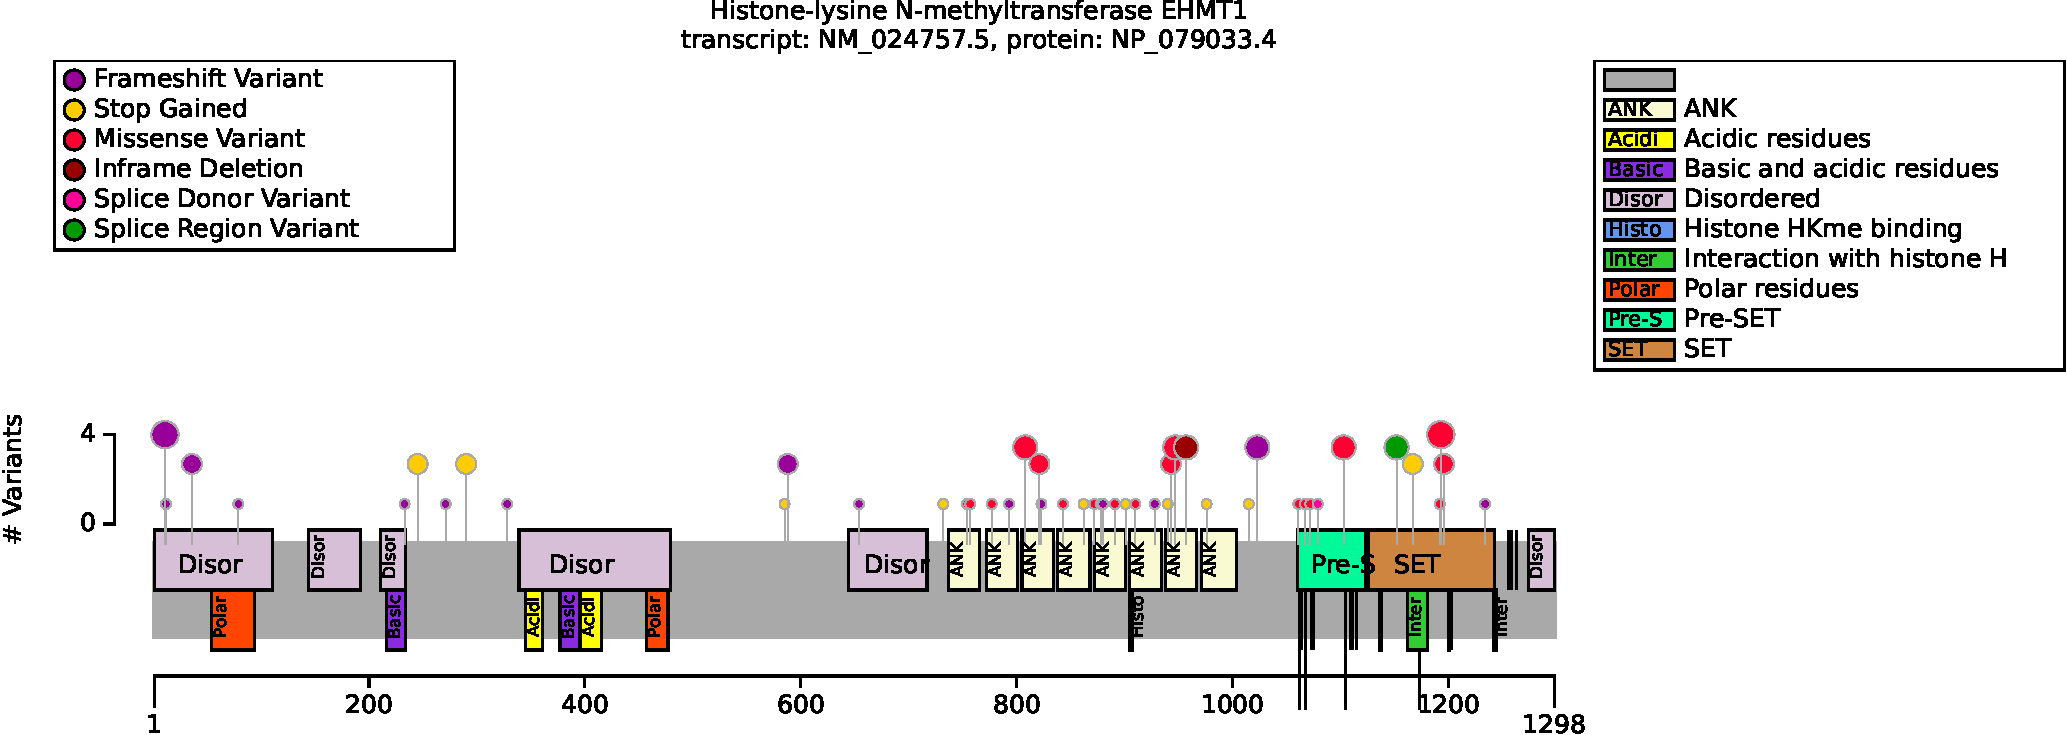
\includegraphics[width=\textwidth]{ img/EHMT1_protein_diagram.pdf} 
\captionsetup{justification=raggedright,singlelinecheck=false}
\caption{Distribution of variants in EHMT1}
\end{subfigure}

\vspace{2em}

\begin{subfigure}[b]{0.95\textwidth}
\centering
\resizebox{\textwidth}{!}{
\begin{tabular}{llllrr}
\toprule
HPO term & N Term Frameshift & other & p-value & adj. p-value\\
\midrule
Attention deficit hyperactivity disorder [HP:0007018] & 4/8 (50\%) & 3/96 (3\%) & $4.83\times 10^{-4}$ & 0.029\\
\bottomrule
\end{tabular}
}
\captionsetup{justification=raggedright,singlelinecheck=false}
\caption{Fisher Exact Test performed to compare HPO annotation frequency with respect to N Term Frameshift and other. Total of
        60 tests were performed.}
\end{subfigure}
\vspace{2em}
\begin{subfigure}[b]{0.95\textwidth}
\centering
\resizebox{\textwidth}{!}{
\begin{tabular}{llllrr}
\toprule
Genotype (A) & Genotype (B) & total tests performed & significant results\\
\midrule
Missense & Other & 62 & 0\\
FEMALE & MALE & 62 & 0\\
ANKR & other & 62 & 0\\
SET & other & 62 & 0\\
\bottomrule
\end{tabular}
}
\captionsetup{justification=raggedright,singlelinecheck=false}
\caption{Fisher Exact Test performed to compare HPO annotation frequency with respect to genotypes. }
\end{subfigure}

\vspace{2em}

\caption{ The cohort comprised 125 individuals (81 females, 44 males). A total of 60 HPO terms were used to annotate the cohort. Disease diagnosis: Kleefstra syndrome 1 (OMIM:610253). 
Rots et al. reported several correlations \cite{PMID_39013458}. Multiple-testing correction was not performed. Frazier et al (2025) also reported significant correlations but the original data was not made available \cite{PMID_39746677}.  A total of 62 unique variant alleles were found in \textit{EHMT1} (transcript: \texttt{NM\_024757.5}, protein id: \texttt{NP\_079033.4}).}
\end{figure}
